\documentclass[pdftex,twocolumn,9pt,letterpaper]{extarticle}


%%% Set these variables appropriately
%%%
%% Note:  Authors is hardcoded below, this line only used for the PDF info
\newcommand{\AUTHORS}{Sarthak Grover, Anna-Kaisa Pietilainen, Renata Tiexiera,
Christian Kreibich, Nick Feamster}
\newcommand{\TITLE}{Detecting Home Network Bottlenecks}
\newcommand{\KEYWORDS}{Put your keywords here}
\newcommand{\CONFERENCE}{Somewhere}
\newcommand{\PAGENUMBERS}{no}       % "yes" or "no"
\newcommand{\COLOR}{yes}
\newcommand{\showComments}{yes}
\newcommand{\comment}[1]{}
\newcommand{\onlyAbstract}{no}


%%%%%%%%%%%%%%%%%%%%%%%%%%%%%%%%%%%%%%%%%%%%%%%%%%%%%%%%%%%%%%%%%%%%%
% ACM Fonts

\newfont{\secfnt}{ptmb8t at 12pt}
\newfont{\secit}{ptmbi8t at 12pt}    %13 Jan 00 gkmt
\newfont{\subsecfnt}{ptmri8t at 11pt}
\newfont{\subsecit}{ptmbi8t at 11pt}  % 
\newfont{\ttlfnt}{phvb8t at 18pt}
\newfont{\ttlit}{phvbo8t at 18pt}    % GM 2/4/2000
\newfont{\subttlfnt}{phvr8t at 14pt}
\newfont{\subttlit}{phvro8t at 14pt} % GM 2/4/2000
\newfont{\subttlbf}{phvb8t at 14pt}  % 13 Jan 00 gkmt
\newfont{\aufnt}{phvr8t at 12pt}
\newfont{\auit}{phvro8t at 12pt}     % GM 2/4/2000
\newfont{\affaddr}{phvr8t at 10pt}
\newfont{\affaddrit}{phvro8t at 10pt} % GM 2/4/2000
\newfont{\eaddfnt}{phvr8t at 12pt}
\newfont{\ixpt}{ptmr8t at 9pt}
\newfont{\confname}{ptmri8t at 8pt}
\newfont{\crnotice}{ptmr8t at 8pt}
\newfont{\ninept}{ptmr8t at 9pt}

%%%%%%%%%%%%%%%%%%%%%%%%%%%%%%%%%%%%%%%%%%%%%%%%%%%%%%%%%%%%%%%%%%%%%%

\hyphenation{off-load-ing}

%%%%%%%%%%%%%%%%%%%%%%%%%%%%%%%%%%%%%%%%%%%%%%%%%%%%%%%%%%%%%%%%%%%%%

%%%
%%%  Page Setup
%%%
\special{papersize=8.5in,11in}
\setlength{\pdfpagewidth}{8.5in}
\setlength{\pdfpageheight}{11in}

\usepackage{ifthen}
\ifthenelse{\equal{\PAGENUMBERS}{yes}}{%
\usepackage[nohead,
% SIGCOMM?
            left=0.75in,right=0.85in,top=0.75in,
% USENIX
%            left=1.0in,right=1.0in,top=1.0in,
            footskip=0.5in,bottom=1.0in,     % Room for page numbers
            columnsep=0.33in
%            columnsep=0.2in  %SPACE
            ]{geometry}
}{%
\usepackage[noheadfoot,left=0.75in,right=0.85in,top=0.75in,
            footskip=0.5in,bottom=1in,
            columnsep=0.25in
	    ]{geometry}
}

%%%
%%%  Captions
%%%
%\usepackage[font=bf]{caption}
\usepackage[font=small,format=plain,labelfont=bf,textfont=it,aboveskip=4pt]{caption}

%%  Space between figure and caption (assuming caption
%%  is below figure)
%\usepackage[font=bf,aboveskip=0pt]{caption} % SPACE
%%  Space between caption and body text of document
\addtolength{\textfloatsep}{-7pt} % SPACE

%%%
%%%  Section headings
%%%
%\usepackage{titlesec}
%\titlespacing{\paragraph}{0pt}{*1}{*1}      % SPACE
\usepackage[compact]{titlesec}              % SPACE
%\titleformat{\section}%                     % IEEE/ACM: caps + period
%  {\bf\large\uppercase}{\thesection.\quad}{0pt}{}

%%%
%%%  Lists
%%%
\usepackage{paralist}
\usepackage{enumitem}
\setlist{itemsep=0pt,parsep=0pt}             % more compact lists

\renewcommand{\paragraph}[1]{\vspace*{0.03in}\noindent{\bf #1}}

%%%
%%% Custom Environments
%%%

\usepackage{balance}
\usepackage{subcaption}
\usepackage{amsmath, amssymb,alltt}
\usepackage{url,tabularx,amsmath,amssymb,psfrag,times,multirow,color}
\usepackage{balance}
\usepackage{listings}
\usepackage{algorithm}
\usepackage{algorithmic}
\usepackage{times}
\usepackage{ifthen}
\usepackage[color]{changebar}
\usepackage{marginnote}
\usepackage{amsthm}
\usepackage{textcomp}
\usepackage{graphicx}


%\renewenvironment{itemize}
%{\begin{list}{$\bullet$}{
%    \setlength{\labelsep}{4pt}
%    \setlength{\labelwidth}{3pt}
%    \setlength{\rightmargin}{0pt}
%    \setlength{\leftmargin}{0pt}
%    \addtolength{\leftmargin}{\labelwidth}
%    \addtolength{\leftmargin}{\labelsep}
%}}{\end{list}}

\definecolor{steel_blue}{RGB}{70, 130, 180}

\lstset{
basicstyle=\footnotesize\ttfamily\small,
frame=none,
language=Python,
numbers=none,
breaklines=true,
xleftmargin=0pt
}


\lstdefinelanguage{Pyretic}
{keywords={>>, >+, +, &, push, if_, elif_, else, pop, match, fwd, modify, set, mod, drop, $\triangleleft$, announce, withdraw}, 
  sensitive=true, alsoletter={-,>>,+,&,|,_},comment=[l][\footnotesize\sffamily\textbf]{\!}
}

\lstset{emph={View1, CA, CA-IN, as-path, med, no-prepend},
  keywordstyle=\color{steel_blue}\textbf}
\lstset{language=Pyretic}


%%%
%%%  Header / Footer
%%%
\usepackage{fancyhdr}
\renewcommand{\headrulewidth}{0pt}

\ifthenelse{\equal{\PAGENUMBERS}{yes}}{%
  \pagestyle{plain}
}{%
  \pagestyle{empty}
}

%%%
%%%  Bibliography
%%%
%\usepackage{cite}
\usepackage[numbers,sort]{natbib}

%%%
%%%  Footnotes / Endnotes
%%%
\interfootnotelinepenalty=10000  % Split footnotes are annoying

% If you want endnodes, uncomment:
%\usepackage{endnotes}
%\usepackage{drafthead}
%\let\footnote=\endnote

%%%
%%%  Tables
%%%
\usepackage{booktabs}
\usepackage{color}
\usepackage{colortbl}
\usepackage{float}                           % Must appear before hyperref to
                                             % avoid weird PDF compile issues

%%%
%%%  Fonts
%%%
\usepackage{mathptmx}                        % Times/Times-like math symbols
%\usepackage{courier}
\usepackage[scaled=0.92]{helvet}

%%%
%%%  PDF setup
%%%
\usepackage[breaklinks=true,filecolor=black,citecolor=blue,urlcolor=black,linkcolor=blue,colorlinks,pdfpagelabels,pdfpagelayout=SinglePage]{hyperref}
%\renewcommand\UrlFont{\rmfamily\itshape}

\if 0
\renewcommand*{\backref}[1]{}
\renewcommand*{\backrefalt}[4]{
   \ifcase #1 %
     (Not cited.) %
   \or
     {\small\sffamily (Cited on page~#2.)}%
   \else
     {\small\sffamily (Cited on pages~#2.)}%
   \fi
 }
\renewcommand*{\backrefsep}{, }
\renewcommand*{\backreftwosep}{ and~}
\renewcommand*{\backreflastsep}{ and~}
\fi

\hypersetup{%
pdfauthor = {\AUTHORS},
pdftitle = {\TITLE},
pdfsubject = {\CONFERENCE},
pdfkeywords = {\KEYWORDS},
bookmarksopen = {true}
}

%%
%% Figure placeholder macros
%%

\definecolor{placeholderbg}{rgb}{0.85,0.85,0.85}
\newcommand{\placeholder}[1]{%
\fcolorbox{black}{placeholderbg}{\parbox[top][1.5in][c]{0.95\columnwidth}{#1}}}


%%%
%%%  Misc
%%%

%\setlength{\parindent}{0pt}
%\setlength{\parskip}{\baselineskip}

\clubpenalty=10000  % Don't allow orphans
\widowpenalty=10000 % Don't allow widows

%%%
%%%  To appear/appeared in text on title page
%%%
\usepackage[absolute]{textpos}
\newcommand{\ToAppear}{%
\begin{textblock*}{\textwidth}(0.95in,0.4in)
\begin{flushright}
    %\noindent{\fbox{\textsf{Under submission---please do not
    %redistribute.}}}
    %  --OR--
    \noindent{\small To appear in \textit{Proceedings of the XYZ}\\
    \noindent{\small \textit{Conference (XYZ'08)}, City, State, Month 2008}}
    %  --OR--
    %\noindent{\small In \textit{Proceedings of the XYZ}\\
    %\noindent{\small \textit{Conference (XYZ'08)}, City, State, Month 2008}}
\end{flushright}
\end{textblock*}
}

%%%
%%%  Sample ACM Copyright Block
%%%
\newfloat{acmcr}{b}{acmcr}
\newcommand{\AcmCopyright}{%
\begin{acmcr}
\noindent
\footnotesize
\renewcommand{\baselinestretch}{0.75}
\!\!Permission to make digital or hard copies of all or part of this work
for personal or classroom use is granted without fee provided that
copies are not made or distributed for profit or commercial advantage
and that copies bear this notice and the full citation on the first
page. Copyrights for components of this work owned by others than ACM
must be honored. Abstracting with credit is permitted. To copy
otherwise, or republish, to post on servers or to redistribute to
lists, requires prior specific permission and/or a fee. Request
permissions from permissions@acm.org.  \\
{\em SIGCOMM'14}, August 17--22, 2014, Chicago, IL, USA.\\ 
Copyright 2014 ACM 978-1-4503-2836-4/14/08 ...\$15.00. \\ 
\url{http://dx.doi.org/10.1145/2619239.2626300}
\end{acmcr}
}

%%%
%%% ACM Categories, etc.
%%%


%%%
%%%  Comments
%%%
\newcommand{\note}[2]{
    \ifthenelse{\equal{\showComments}{yes}}{\textcolor{#1}{#2}}{}
}

\newcommand{\xxx}[1]{\note{red}{#1}}

%%%
%%% Abbreviations
%%%
\newcommand{\ie}{{\em i.e.}}
\newcommand{\eg}{{\em e.g.}}
\newcommand{\ea}{{\em et al.}}
\newcommand{\system}{SDX}
\newcommand{\name}{SDX}
\newcommand{\fp}{\vspace*{0.02in}\noindent}

%% \newtheoremstyle{tighter}
%%     {3pt}        % Space above
%%     {3pt}        % Space below
%%     {\em}        % Body font
%%     {}           % Indentation
%%     {\bfseries}  % Head font
%%     {:}          % Head punctuation
%%     {.5em}       % Head space
%%     {}           % Custom head spec
%% \theoremstyle{tighter}
%\newtheorem{lesson}{Lesson}
%\newtheorem{constraint}{Constraint}
%\newcommand{\lesson}[1]{\vspace{1em}{\centering\fbox{\parbox{0.95\columnwidth}{\centering\bf Lesson: #1}}}\vspace{1em}}


\newcommand{\supsym}[1]{\raisebox{4pt}{{\footnotesize #1}}}
\newcommand{\gt}{\supsym{$\dag$}}
\newcommand{\inr}{\supsym{$\diamond$}}
\newcommand{\icsi}{\supsym{$\star$}}
%\newcommand{\ceq}{\supsym{$\ddag$}}
%\newcommand{\usc}{\supsym{$\ddag$}}

\newcommand{\remove}[1]{}
\newcommand{\cmstart}{}
\newcommand{\cmend}{}


\date{}
\title{
%\vspace*{-0.53in}
\textbf{\ttlfnt \TITLE}}
\author{
\aufnt{Sarthak Grover\gt, Anna-Kaisa Pietilainen\inr, Renata Tiexiera\inr,
Christian Kreibich\icsi, Nick Feamster\gt} \\
\gt\affaddr{Georgia Tech}~~~\inr\affaddr{INRIA}~~~\icsi\affaddr{ICSI}
}

%\date{\normalsize\url{http://projectbismark.net}}


% This needs to be the last thing before \begin{document}
\usepackage{microtype}  % SPACE

%%%%%%%%%%%%%%%%%%%%  START DOCUMENT  %%%%%%%%%%%%%%%%%%%%%%%%
\begin{document}

\maketitle

%\AcmCopyright
%\ToAppear

\thispagestyle{empty}

\begin{sloppypar}
\begin{abstract}

Identifying the performance bottleneck in a home network allows for better diagnosis by ISPs, users, and content providers. Existing solutions either troubleshoot network faults, or analyze wireless performance using multiple promiscuous gateways, making them impractical and unscalable in a home network environment consisting of simplistic gateways and wireless devices. Our work presents a highly scalable tool to locate the bandwidth bottleneck (thin link) in a home network from the perspective of the end device. We propose an optimized active measurement approach to estimate the available bandwidth of the wireless (home) and the wireline (access) link by either coordinating with the access point for measurements, or collaborating with other home network devices. Our approach uses bandwidth measurements and timing information from active traffic, and requires no protocol modification, to detect bottlenecks in both wireless network and access link. We evaluate our tool by simulation, on a controlled testbed, and in real home networks. Preliminary results show that our one-shot measurement strategy can accurately detect the bottleneck link within a certain range depending on the variation of wireless and access link bandwidth measurements, either with gateway coordination or by collaborating with another generic device inside the home.

\end{abstract}

\ifthenelse{\equal{\onlyAbstract}{no}}{%

\vspace*{0.1in}
%\fp {\bf Categories and Subject Descriptors:}
%C.2.1 [Computer-Communication Networks] {\em Network Architecture and
%  Design}: Network Communications
%
%\fp {\bf General Terms:}
%Algorithms, Design, Experimentation
%
%\fp
%{\bf Keywords:}
%software defined networking (SDN); Internet exchange point (IXP); BGP
%

\section{Introduction}

Home networks contain a variety of heterogeneous devices competing over the wireless channel for Internet access time. Increasing user demands and ease of accessing content on such wireless devices have resulted in 802.11n, offering datarates as high as 300Mbps. Similarly, there has also been a steady increase in access link capacities to cater to users' high bandwidth requirements. With such high rates many users still face performance issues in home networks, which cannot be pinpointed by simplistic end host bandwidth measurement tools that were not meant for the wireless medium \cite{speedtest}, \cite{netalyzr}.

In our work, we develop an end-host based approach to identify the bottleneck link between the home or on the access network. This information allows ISPs and users to identify whether the bottleneck issue is local or on the access side. Furthermore, content providers such as video hosts (e.g., Netflix) can use this tool to better understand whether lower performance is caused due to local wireless network issues, or because if there was traffic shaping or congestion at the access network side.

Previous research in bottleneck identification has mainly concentrated on tomography \cite{tools}, which were not designed to work on the wireless medium due to its non-work conserving nature. Whereas to study and diagnose the home wireless network, researchers require extra monitoring nodes and kernel changes on the gateway to get an in-depth view into wireless parameters.

A promising method is using collaborative devices, such as the gateway \cite{wtf}, or another wired node in the home \cite{wlanprobe}, to identify the bottleneck. But this approach still requires collaboration with either a highly capable OpenWRT gateway, or a wired computer in the home, both of which are not common current state of the art in home networks. Thus this work has not been tested and evaluated on a large scale. In our work, we progress in this direction by directing the user to use such collaborative measures with other wireless devices available in the home, such as a smartphone.
%Previous research in the domain of bottleneck link identification can be classified into three types.

%\textbf{Tomography:} using packet pair techniques to find the faulty link in an access network based on packet timings at the receiver host \cite{tools}. This approach has not been successfully applied over home networks as they usually contain a wireless links, which are non-work conservative, thereby making timing based approaches statistically prone to error.

%\textbf{Promiscuous nodes or extra antennas:} in the vicinity of the gateway which give a detailed view of the wireless mediums utilization and allow monitoring of radiotap statistics \cite{wise}. These works may also require certain kernel modifications in the gateways to collect erroneous packets. This approach may work well for enterprise networks or laboratories, but is generally impractical and unscalable for home networks, which usually contain just one simple gateway device. 

%\textbf{Gateway collaboration:} allows traffic monitoring from custom firmwares running on home routers and diagnose bottlenecks via passive measurements \cite{wtf}. This approach solves the bottleneck detection problem and has the additional advantage of not introducing any active probing traffic, but it hasn’t been evaluated at scale yet, and requires root access to a capable gateway device inside the home. Similarly, by having a wired device attached to the gateway, one can perform active measurements to diagnose wireless performance by studying delays, as the wired link to the gateway is considered to never be the bottleneck link \cite{wlanprobe}. This approach is the closest to our collaborative solution but requires a wired device collaboration running custom tools inside the home, which is a rare occurrence in today's primarily wireless home networks.
\section{Detection Algorithm}

Our goal is to detect the home network bottleneck in a scalable, easily installable manner, without introducing excessive probing traffic. Furthermore, we can take advantage of collaborative devices in the home, such as smart phones, other laptops, and collaborative gateways (if available). To this end, we present a bandwidth bottleneck detection algorithm. Currently implemented as a python tool, in the future, we will port this algorithm to a browser extension to perform low traffic bandwidth and latency tests.

\subsection{Bandwidth Bottleneck}
\label{bandwidth}

We compare the available TCP bandwidth of individual segments (home, access, end to end) to pinpoint the tight link. Consider that we have an external server to test to, and a wireless test client inside the home. Now, we can perform measurements if either of the two devices are also present: (a) collaborative gateway; (b) user controlled collaborative test device

\textbf{Collaborative Gateway:} which can form an end point for bandwidth measurements
\begin{itemize}[noitemsep,topsep=0pt,parsep=0pt,partopsep=0pt]
\item Measure wireless TCP bandwidth between client and router.
\item Start measuring access TCP bandwidth between router and client.
\item Stop measurement as soon as the access throughput exceeds wireless throughput. If this happens, wireless is bottleneck. Else, access is bottleneck.
\end{itemize}
This algorithm was evaluated in both the testbed and real networks with OpenWRT gateways (Section \ref{evaluation})

\textbf{Collaborative Test Device:} The main idea here is to direct the user to place a control device, such as a smartphone, in the home at a good position ensuring a good wireless throughput, to conduct tests using that device as a reference. %See figure \ref{fig:two-device}
\begin{itemize}[noitemsep,topsep=0pt,parsep=0pt,partopsep=0pt]
\item Place control end host device (B) near home gateway and ensure it has a better throughput than test device (A) to the server (S). Throughput of test device = AS; throughput of control device = BS.
\item Measure bidirectional wireless bandwidth between test and control devices, i.e. throughput AB (or BA).
\item If AS < AB, then access link is bottleneck.%If wireless bandwidth between the two devices (AB) exceeds end to end throughput of test device (AS), then access link is the bottleneck. i.e., 
\item If AS < AB < BS, then wireless link is bottleneck.%%If wireless bandwidth between the two devices (AB) is less than the end to end throughput of control device (BS), but more than the end to end throughput of the test device (AS), then wireless link of test device is the bottleneck. i.e.,
\end{itemize}

%\begin{figure}[!ht]
%\begin{center}
%    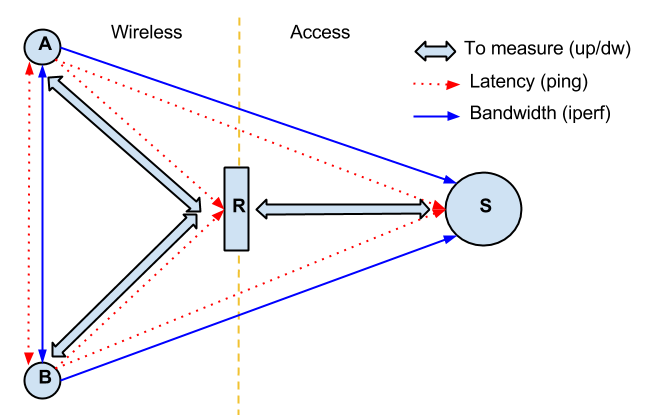
\includegraphics[width=3.2in,height=1.9in]{two-device.png}
%\end{center}
%\caption{Bandwidth and Latency measurements using two collaborating devices.}
%\label{fig:two-device}
%\end{figure}

\subsection{Latency Bottleneck}
\label{latency}

This algorithm is based on the observation that the buffers of a tight link are full during an end to end flow. One way to check for this is to compare the increase in RTT over the home and access segment when a link is being probed. Another approach to detect tight links is by differentially overflowing the wireless and the access link and comparing the delay observed at the listener. This can be done using STAB \cite{stab}, a successor of the pathChirp \cite{pathchirp}.

We use one end host device to send a train of pairs of large packets followed immediately by a small packet . The large packet has a limited TTL and is dropped at a particular hop based on that TTL. So it only saturates the link before it was dropped. The listener (end host server) records the timing of the small packet to diagnose the thin bottleneck link at which the big packet with limited TTL got dropped. If the access link is the uplink bottleneck, we will see that TTL=1 packets which only saturate the wireless result in smaller timings at the listener than the packet trains with large TTL which also covers the access network.
\section{Evaluation}
\label{evaluation} 
In this section, we evaluate the algorithms proposed on a controlled testbed.

Our experimental tests were performed using two lenovo T430 laptops running debian (A and B), a BISmark access gateway \cite{sundaresan2011broadband} that has an OpenWRT-based platform for performing measurements (R), an OpenWRT-router used as a control router to limit access uplink and downlink bandwidth (Q), and a server machine with access to the Internet, running debian (S). Our experiments confirmed that TCP throughput over each link can be accurately measured to 90\% of the capacity using 4 parallel threads with a duration of 5 seconds.

We use a custom tc script with netem \cite{netem} on the control router to change access link bandwidth settings, and distance the wireless clients (A and B) to control the wireless channel. Our results indicate that the bandwidth based algorithms presented in \ref{bandwidth} can find the bottleneck accurately within 3 Mbps (Fig. \ref{fig:throughput_vs_bottleneck}).

\begin{figure}[!ht]
  \centering
  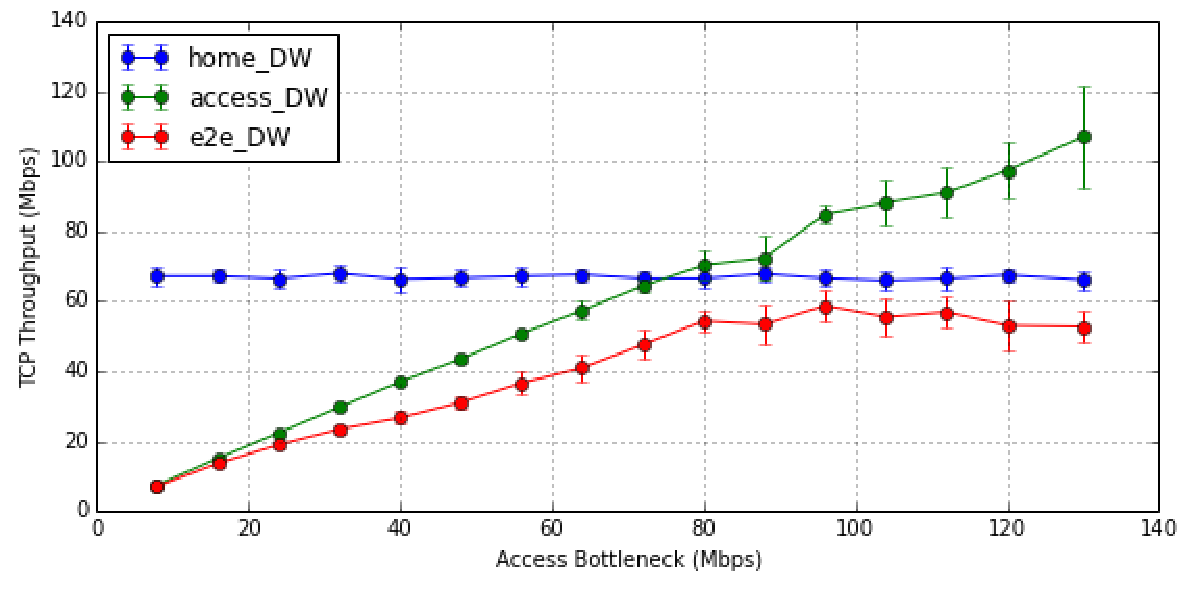
\includegraphics[width=\linewidth]{figures/tcp_throughput_vs_bottleneck}
  \caption{Bandwidth measured over each link for a wireless client with a good channel while varying the access link bottleneck}
  \label{fig:throughput_vs_bottleneck}
\end{figure}


%\begin{figure}[!ht]
%\begin{minipage}{.5\textwidth}
%  \centering
%  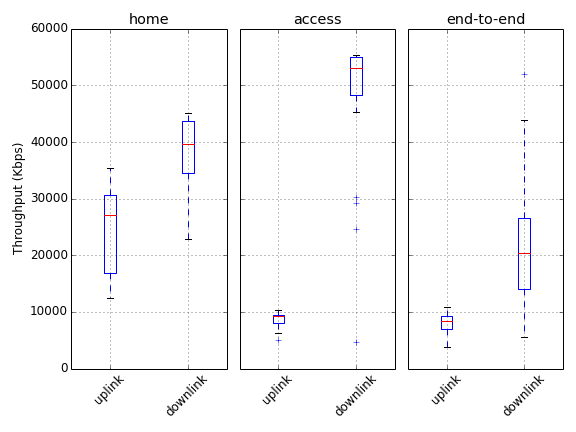
\includegraphics[width=.4\linewidth]{figures/boxplot_throughput.png}
%  \captionof{figure}{Bandwidth measurements}
%  \label{fig:bandwidth}
%\end{minipage}%
%\begin{minipage}{.5\textwidth}
%  \centering
%  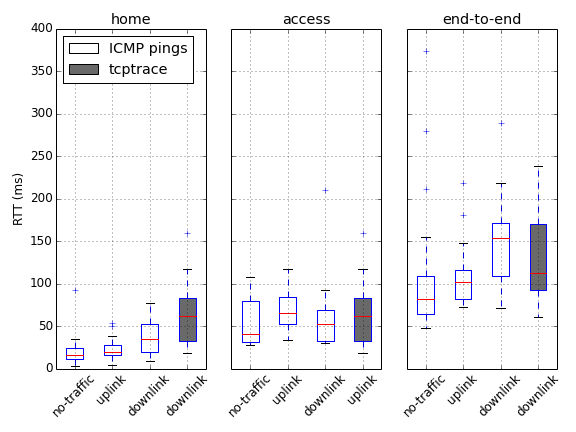
\includegraphics[width=.4\linewidth]{figures/boxplot_latency.png}
%  \captionof{figure}{Latency measurements (confirmed using tcptrace)}
%  \label{fig:latency}
%\end{minipage}
%\end{figure}

%\begin{figure}[!ht]
%  \centering
%  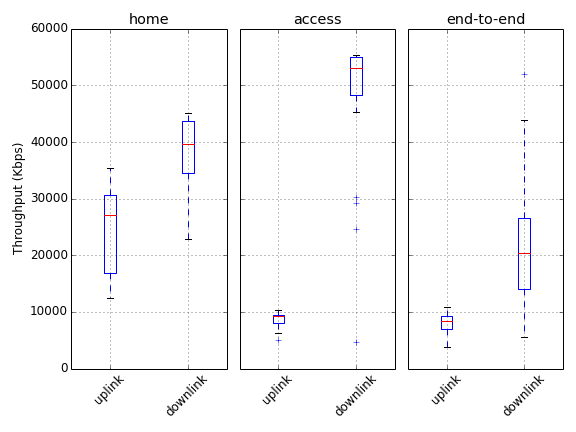
\includegraphics[width=\linewidth]{figures/boxplot_throughput.png}
%  \caption{Bandwidth measurements}
%  \label{fig:bandwidth}
%\end{figure}
\balance\section{Future Work}
The current solution is a python based script running on the client device which performs bandwidth and latency measurements using tools such as iperf. It uses RPC to communicate with the gateway and publishes commands to an open script port on the server device. We perform the analysis offline after collecting data.

Our next step is to test the advanced latency based diagnosis method detailed in section \ref{latency} to gain an understanding of the reason for a wireless bottleneck.

Next, we will port the developed bottleneck detection approach to a browser as an extension, making it highly scalable, and easily installable, on the multitude of heterogeneous devices available in a home network. Further, we aim to evaluate our solution for public wifi networks where there are many competing wireless devices and no access to the wireless gateway at all.

As an extension of our work, we would like to explore the reasons behind a wireless bottleneck and suggest simple solutions to the user if possible. We will start by creating different kinds of wireless and home bottlenecks, such as interference, low power, congestion at the router, and hidden terminals. Then, using additional monitoring antennas at the router, we would like to find if we can detect this, and relate it to the more common case where we have only a second collaborating device. Gaining inspiration from \cite{wlanprobe}  we have started by looking at packet delays at the listener using an approach similar to that presented in Section \ref{latency}.
%\label{lastpage}
\end{sloppypar}

%\appendix
%\input{appendix_sources}

%\vspace{-0.1in}
%\section*{Acknowledgments}
%We thank our shepherd Walter Willinger, Hyojoon Kim, Jo\~ao Lu\'is Sobrinho,
%Jennifer Gossels, Darrell Newcomb, Michael Schapira, and the anonymous reviewers for
%comments.  This research was supported by NSF awards CNS-1040705,
%CNS-1040838, CNS-1162112, CNS-1261462, and CNS-1261357.  We thank
%Internet2 for their support and recognition with an Internet Innovation Award, the
%organizations that host Transit Portal nodes, and the GENI Project Office
%for supporting our ongoing deployment efforts.

%% Bibliography

%\pagebreak
\setlength{\bibsep}{0pt}
\small
\bibliographystyle{abbrv}
\flushleft\balance\bibliography{paper}  % sigproc.bib is the name of the
                                % Bibliography in this case 
%\bibliographystyle{abbrvnat_noaddr} % SPACE
%\theendnotes % ENDNOTES
}{% !onlyAbstract
}

\end{document}

% Local Variables:
% TeX-command-default: "LaTeX PDF"
% End: